\section{Technical Part}

\renewcommand{\labelenumi}{\alph{enumi}.}

\subsection{Plotting and Downsampling}
\begin{enumerate}
  \item The original sampling rate is \textbf{48 (KHz)}.
  \item There are missing timeframes in the pitch where there isn't a voiced phonation.
  \item The scipy downsampling would sound better. 
  By the Nyquist theorem naive downsampling by 2 halves the maximum frequency that can be represented.
  If our signal contains a frequency greater than $\frac{32}{2}=16$ KHz it would be aliased, disrupting the signal.
  The scipy method applies the FFT to the signal and then removes frequencies that would be aliased before resampling.
  My recording does not contain significant frequencies above 16KHz, so both methods sound similar. 
\end{enumerate}


\subsection{Spectral Noise Subtraction}

\subsubsection{Adding Noise}
Below are the 3 plots corresponding to the original (downsampled) signal, the noise and the noised signal.
\begin{figure}[h]
  \centering
  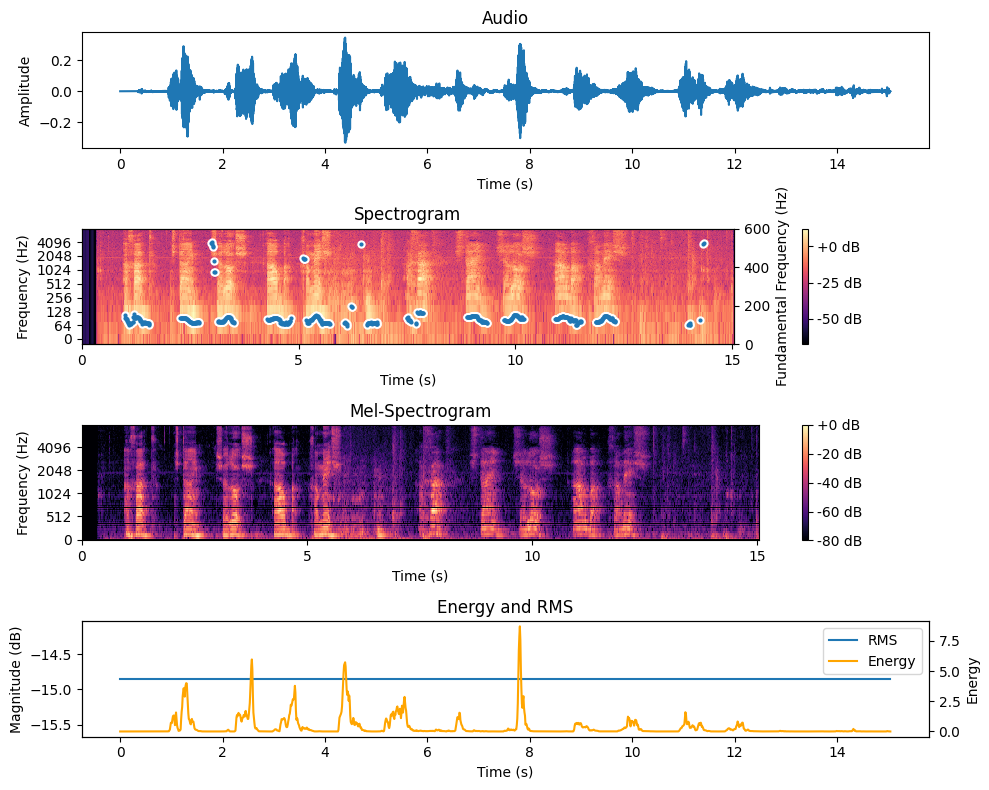
\includegraphics[width=0.9\textwidth]{downsampled_clean_plot.png}
  \caption{The clean (downsampled) signal plot.}
\end{figure}

\begin{figure}
  \centering
  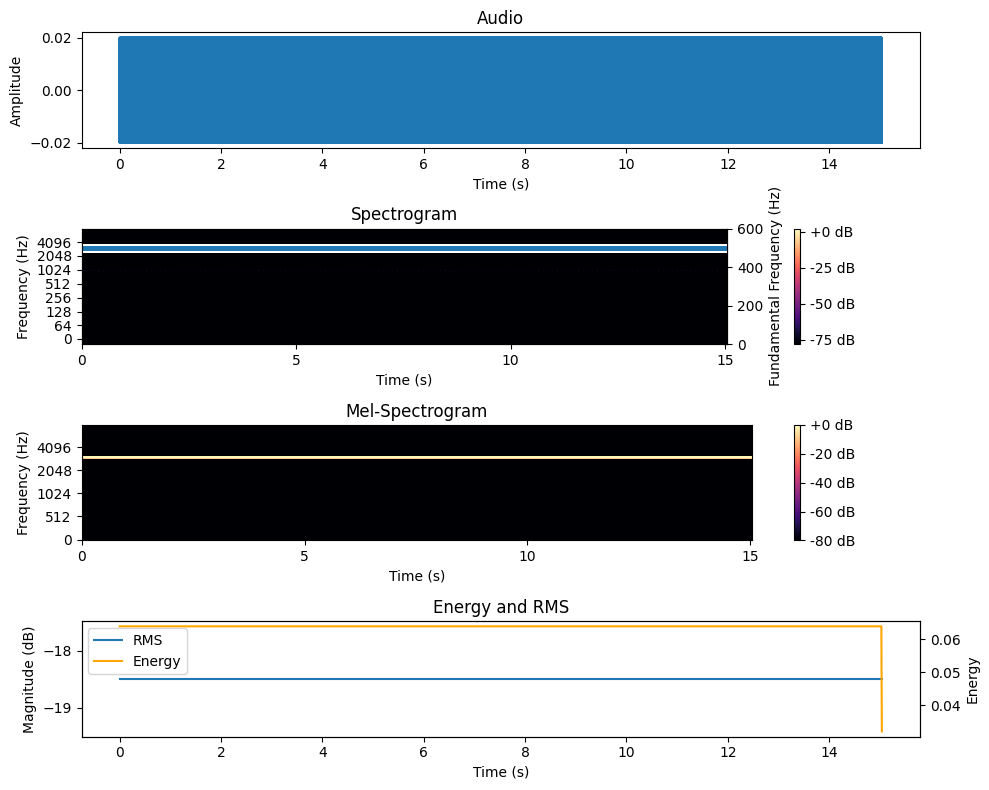
\includegraphics[width=0.9\textwidth]{noise_plot.png}
  \caption{The additive noise plot.}
\end{figure}

\begin{figure}
  \centering
  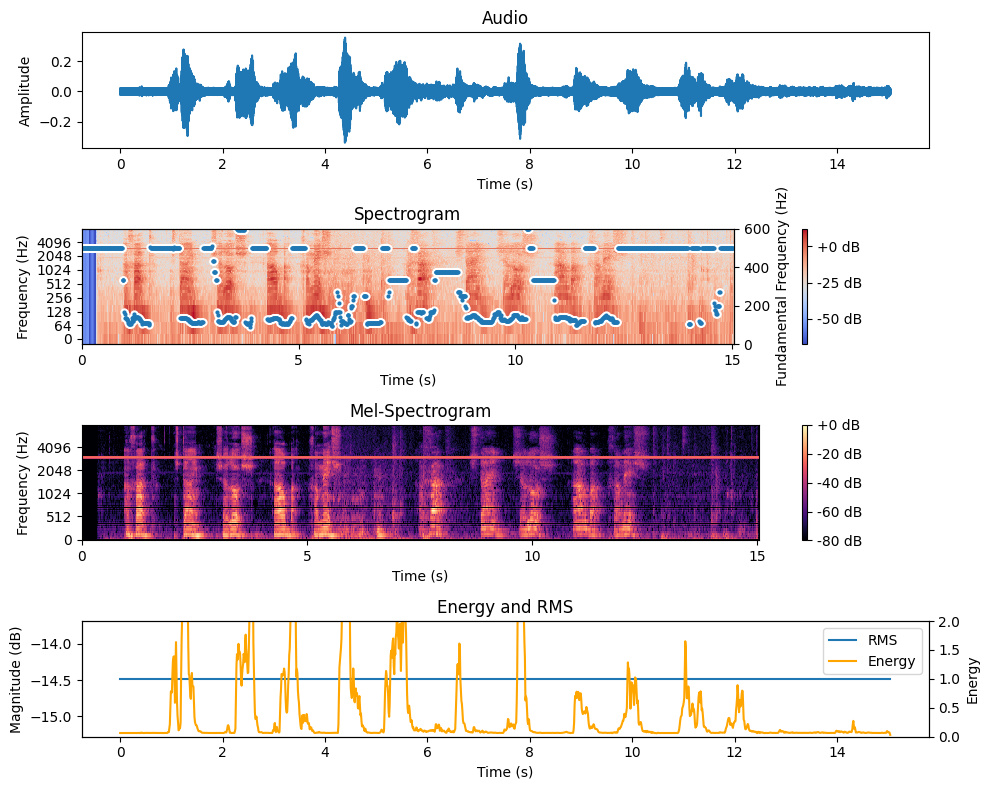
\includegraphics[width=0.9\textwidth]{noised_downsampled_plot.png}
  \caption{The noised signal plot.}
\end{figure}

\subsubsection{Spectral Substraction}
\begin{enumerate}
  \item The energy threshold plot for voice activity detection is seen in Figure 4.
  \begin{figure}
    \label{fig:VAD}
    \centering
    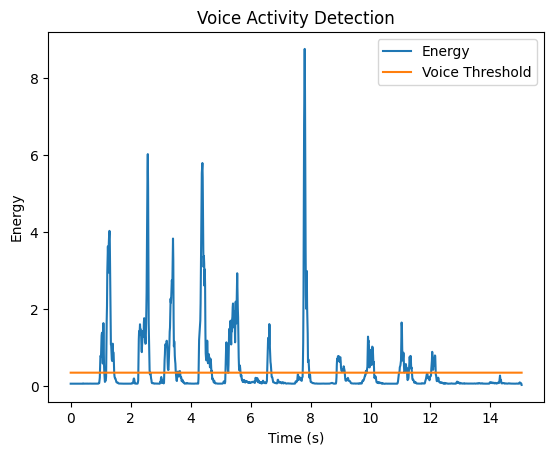
\includegraphics[width=0.64\textwidth]{voice_avctivity_detection.png}
    \caption{Energy contour plot with threshold for VAD}
  \end{figure}

  \item The plot for the denoised audio using spectral subtraction is given in Figure 5.
  \begin{figure}[b]
    \label{fig:denoised_plot}
    \centering
    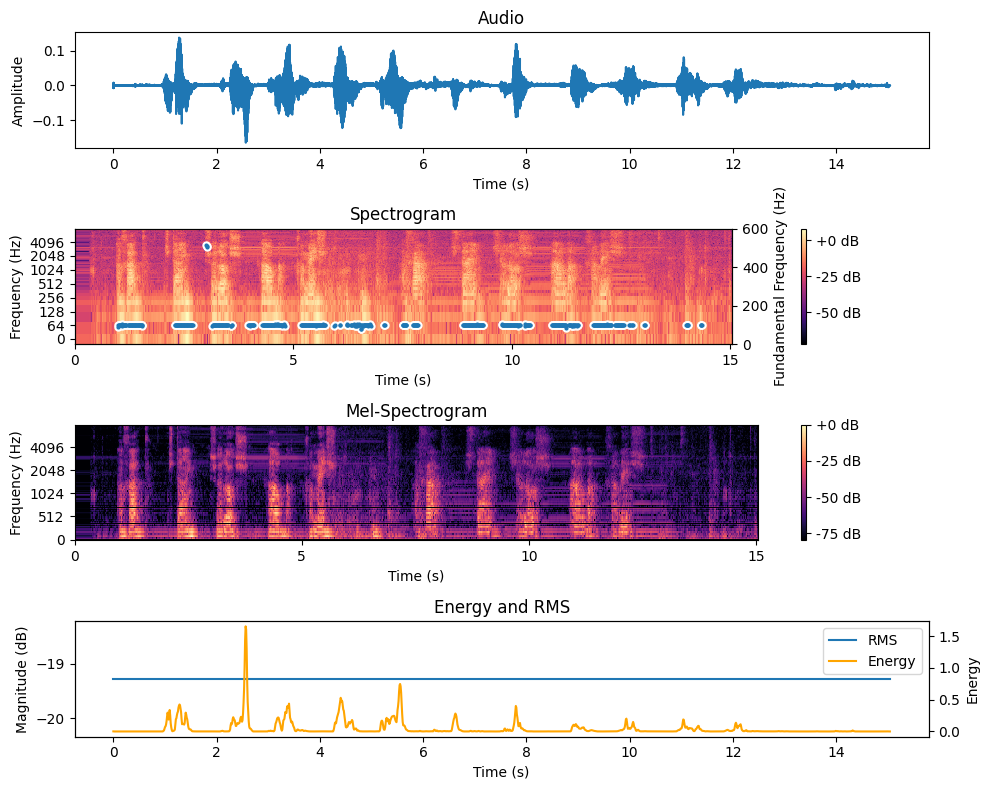
\includegraphics[width=0.9\textwidth]{cleand_audio_plot.png}
    \caption{Audio plot of the denoised signal.}
  \end{figure}
\end{enumerate}

\subsubsection{Auto Gain Control}
\begin{enumerate}
  \item The desired RMS was chosen to be \textbf{-20 dB} and the noise floor threshold was chosen to be \textbf{-46 dB}.
  Figure 6 shows the rms over time and the selected thresholds.
  \begin{figure}
    \label{fig:agc_rms}
    \centering
    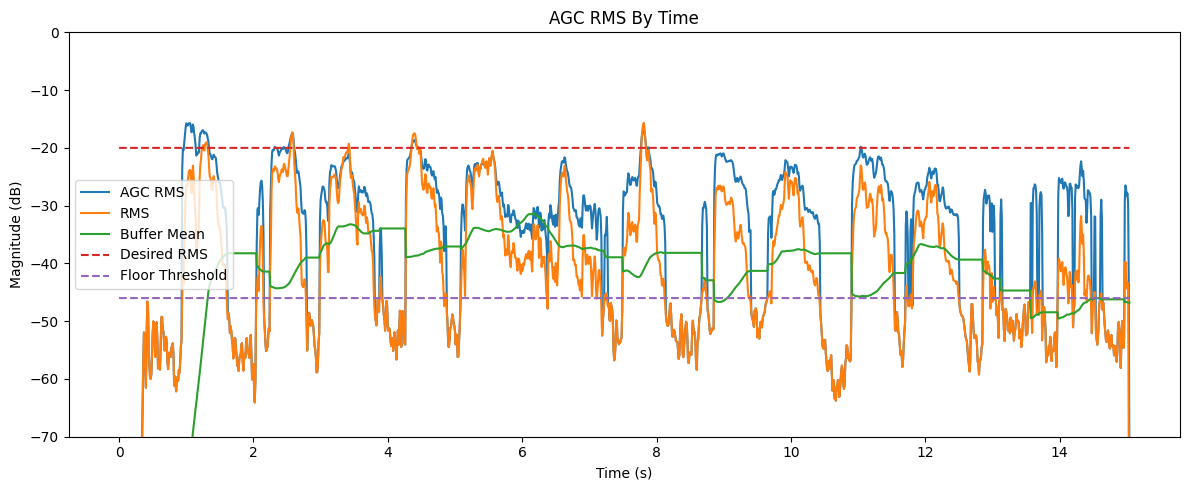
\includegraphics[width=0.9\textwidth]{agc_rms_full.png}
    \caption{RMS values for the AGC enhanced signal.}
  \end{figure}
  
  \item We plot the AGC enhanced signal in Figure 7.
  \begin{figure}
    \label{fig:agc_plot}
    \centering
    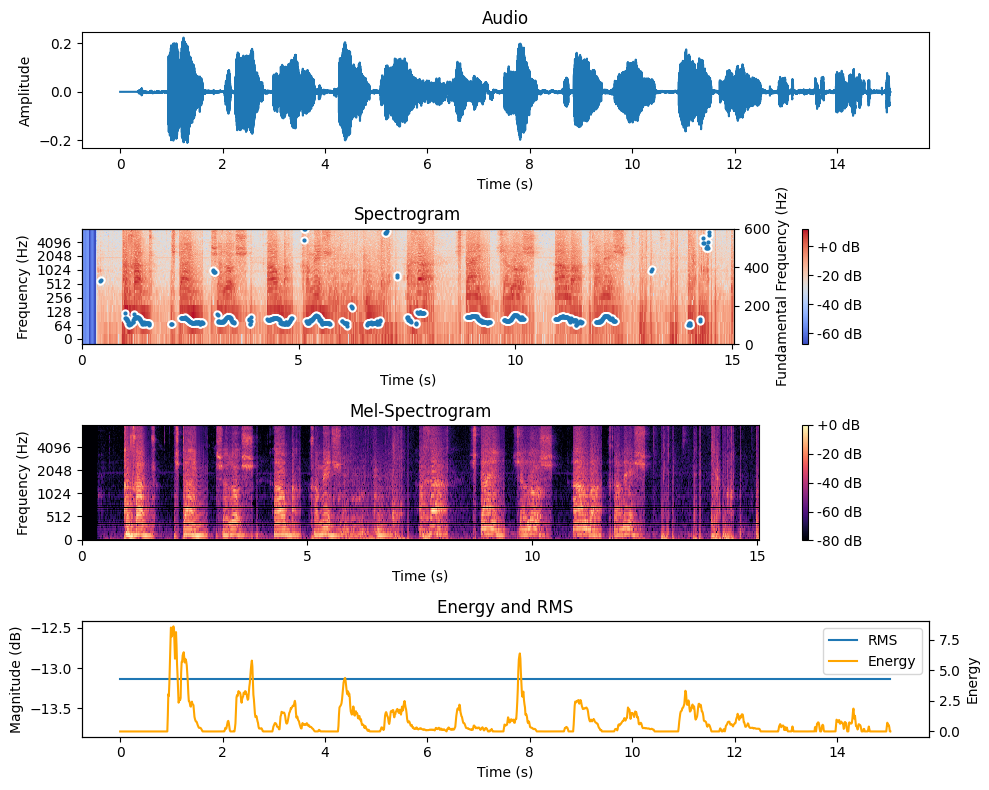
\includegraphics[width=0.9\textwidth]{agc_plot.png}
    \caption{Audio plot for the AGC enhanced signal.}
  \end{figure}

  \item The scaling factor plot is shown in Figure 8. 
  We used the metric of dB relative to reference amplitude of 1, as used in librosa.
  Note that for negative amplitude values a scaling factor lower than 1 corresponds to an increase of amplitude, a scaling factor of 1 corresponds to no change to the amplitude (such as when no voice is detected) and a factor greater than 1 corresponds to a decrease in amplitude.
  \begin{figure}
    \label{fig:scaling_factor}
    \centering
    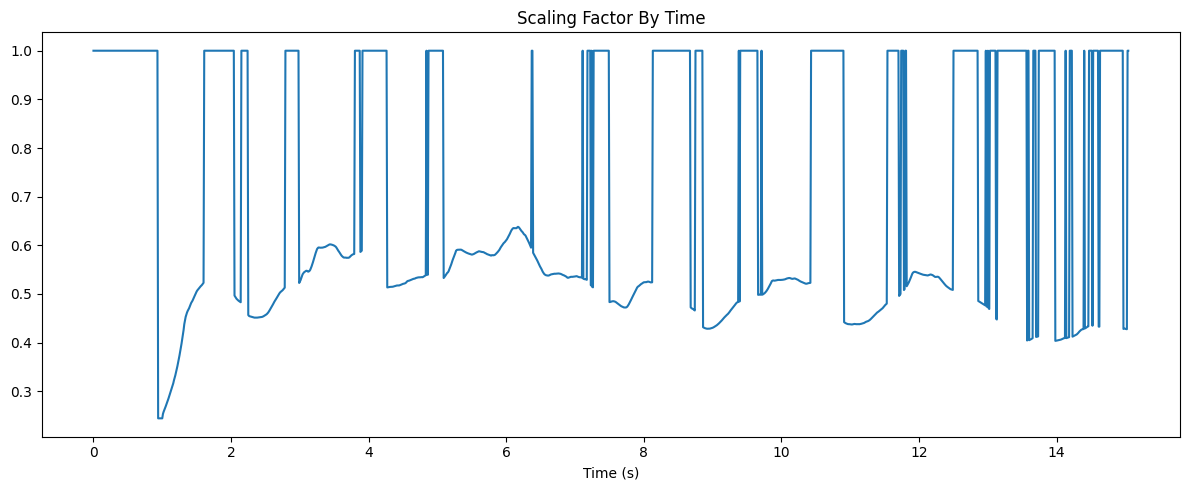
\includegraphics[width=0.9\textwidth]{agc_scaling_factor.png}
    \caption{Audio plot for the AGC enhanced signal.}
  \end{figure}

\end{enumerate}